\chapter{Numeri relativi}
\label{sha:numerirelativi}
\minitoc
\mtcskip                                % put some skip here
\minilof                                % a minilof
\mtcskip                                % put some skip here
\minilot
\section{Glossario}
\begin{figure}
	\centering
	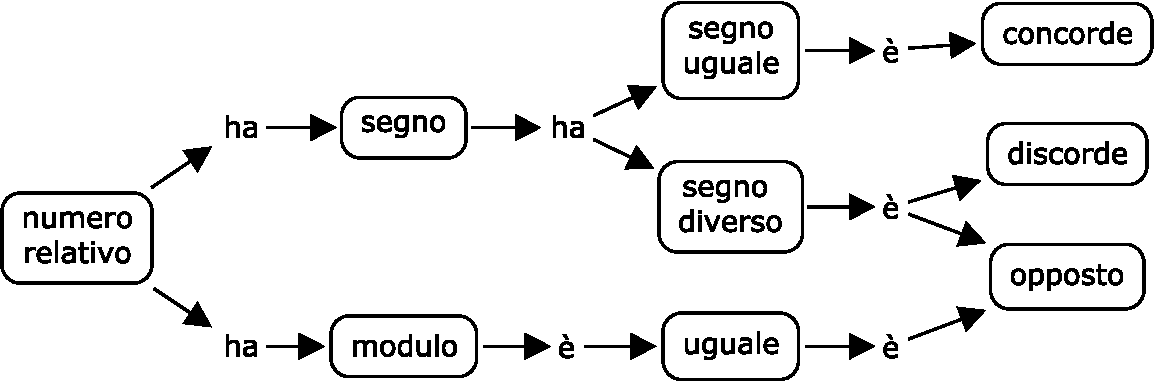
\includegraphics[scale=0.5]{numerirelativi-crop}
	\caption{Numeri relativi}
	\label{fig:numORealativi}
\end{figure}
\begin{enumerate}
	\item Un numero relativo è formato da una parte numerica detta modulo e da un segno
	\item Due o più numeri relativi che hanno lo stesso segno si dicono concordi
	\item Due o più numeri relativi che hanno  segno diverso si dicono discordi
	\item Due numeri relativi concordi che hanno lo stesso modulo si dicono opposti.
\end{enumerate}
\section{Ordine}
Ordinare dei numeri significa confrontali fra di loro per stabilire un prima e un poi. La figura\nobs\vref{fig:ordinamentonumrel} è un esempio di ordinamento. In questo ordine i numeri negativi sono a sinistra dello zero e i numeri positivi a destra. 

Quando ordiniamo due numeri relativi possiamo avere tre casi
\begin{enumerate}
	\item I due numeri sono concordi positivi: In questo caso è maggiore il numero con modulo più grande;
	\item I due numeri sono concordi negativi: In questo caso è maggiore il numero con modulo più piccolo;
	\item  I due numeri sono discordi: In questo caso è maggiore il numero positivo;
\end{enumerate}
\begin{figure}[!t]
	\centering
	\begin{tikzpicture}[>=triangle  45]
	\draw [->](-7,0)--(7,0);
	\foreach \x in {-7,-6,...,7}
	\draw (\x,0) -- (\x,-.1) node[below] {$\x$};
	%\node (a) at (\x,0.6) {$\x$};
	\end{tikzpicture}
	\caption{Ordinamento}
	\label{fig:ordinamentonumrel}
\end{figure}
\section{Operazioni con i numeri relativi}
\label{sec:Operazioniconnumerirelativi}
I numeri relativi sono formati da due parti, quindi un'operazione deve definire delle regole che permettano di determinare il segno e il modulo del risultato.
\subsection{Somma sottrazione}
La somma di due numeri relativi segue le sue regole che sono simili a quelle della moltiplicazione ma con cui non vanno confuse.

Quando sommiamo due numeri relativi possiamo avere cinque casi come nel seguente esempio:
\begin{itemize}
	\item $+5+3=+8$: I due numeri hanno lo stesso segno e come risultato ho un numero dello stesso segno e che ha per modulo la somma dei moduli
	\item $-5-3=-8$: I due numeri hanno lo stesso segno e come risultato ho un numero dello stesso segno e che ha per modulo la somma dei moduli
	\item $-5+3=-2$: I due numeri hanno segno diverso e come risultato ho un numero dello stesso segno del numero maggiore in modulo e che ha per modulo la differenza dei moduli
	\item $+5-3=+2$: I due numeri hanno segno diverso e come risultato ho un numero dello stesso segno del numero maggiore in modulo e che ha per modulo la differenza dei moduli
	\item $+5-5=0$: I due numeri sono opposti e come risultato ottengo zero.
\end{itemize}
\subsection{Prodotto}
Quando moltiplico due numeri posso avere due casi:
\begin{itemize}
	\item I due numeri sono concordi ottengo un numero positivo.
	\item I due numeri sono discordi ottengo un numero negativo.
\end{itemize}
\subsection{Divisione}
Quando divido due numeri posso avere due casi:
\begin{itemize}
	\item I due numeri sono concordi ottengo un numero positivo.
	\item I due numeri sono discordi ottengo un numero negativo.
\end{itemize}
\subsection{Potenze}
\begin{table}[H]
	\centering
	\begin{tabular}{RCL}
		\toprule
		a^n&=&\overbrace{a\times a\times\cdots\times a}^{n{}\mbox{volte}}\\[.6cm]
		a^0&=&1\\[.6cm]
		0^0&=&?\\[.6cm]
		a^n\cdot a^m&=&a^{n+m}\\[.6cm]
		a^m\div a^n&=&a^{m-n}\text{ se }m\geq n\\[.6cm]
		\left(a^n\right)^m&=&a^{n\cdot m}\\[.6cm]
		a^{n}b^{n}&=&{\left(ab\right)}^n\\[.6cm]
		a^{n}\div b^{n}&=&{\left(a\div  b\right)}^n\\[.6cm]
		\left(\dfrac{a}{b}\right)^n&=&\dfrac{a^n}{b^n}\\[.6cm]
		a^{-n}&=&\left(\dfrac{1}{a}\right)^n\\
		
		\bottomrule
	\end{tabular}
	\caption{Proprietà delle potenze}
\end{table}